\documentclass[UFT8]{beamer}
\usepackage{tikz}
\usetikzlibrary{arrows, positioning, shapes.geometric, arrows.meta}

\mode<presentation> {
	\usetheme{Frankfurt}
	% or AnnArbor Antibes Bergen Berkeley Berlin Boadilla boxes CambridgeUS Copenhagen Darmstadt default Dresden Frankfurt Goettingen Hannover Ilmenau JuanLesPinsLuebeck Madrid Malmoe Marburg Montpellier PaloAlto Pittsburgh Rochester Singapore Szeged Warsaw
	
	\setbeamercovered{transparent}
	% or whatever (possibly just delete it)
}

\usepackage{color}
\usepackage{algorithm,algpseudocode}
\usepackage{algorithmicx}
\usepackage{algpseudocode}
\usepackage{amsmath}
\usepackage{float}

\usefonttheme[onlymath]{serif}

% \documentclass[ppt.tex]{subfiles}
\begin{document}

\section{{Proof System}}

\begin{frame}
    \frametitle{Public Coin and Fiat-Shamir Transformation}
	\begin{itemize}
		\item Claim: $x \in \mathcal{L}$
	\end{itemize}

	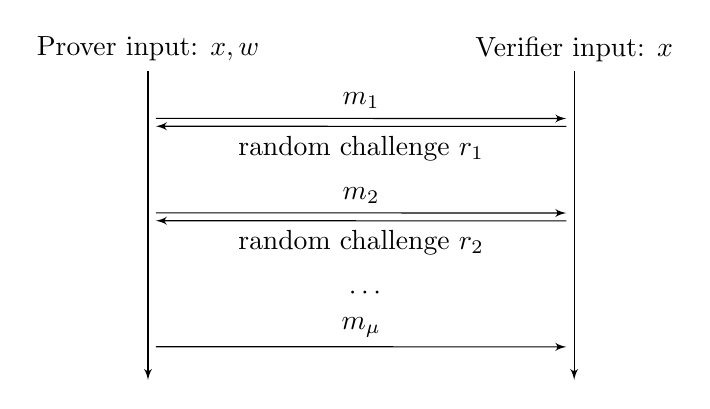
\begin{tikzpicture}[auto, node distance=2.5cm,>=latex']
		\node [rectangle, align=center] (prover) {Prover input: $x, w$};
		\node [rectangle, right=of prover, align=center] (verifier) {Verifier input: $x$};
	
		\draw[->] (prover) -- +(0, -42mm);
		\draw[->] (verifier) -- +(0, -42mm);
	
		\draw[->] ([yshift=-6mm, xshift=1mm]prover.south) -- node {$m_1$} ([yshift=-6mm, xshift=-1mm]verifier.south);
		\draw[->] ([yshift=-7mm, xshift=-1mm]verifier.south) -- node {random challenge $r_1$} ([yshift=-7mm, xshift=1mm]prover.south);
	
		\draw[->] ([yshift=-18mm, xshift=1mm]prover.south) -- node {$m_2$} ([yshift=-18mm, xshift=-1mm]verifier.south);
		\draw[->] ([yshift=-19mm, xshift=-1mm]verifier.south) -- node {random challenge $r_2$} ([yshift=-19mm, xshift=1mm]prover.south);
	
		\path (prover) -- (verifier) node[midway, yshift=-33mm] (ellipsis) {$\cdots$};
	
		\draw[->] ([yshift=-35mm, xshift=1mm]prover.south) -- node {$m_\mu$} ([yshift=-35mm, xshift=-1mm]verifier.south);
	\end{tikzpicture}

	\begin{itemize}
		\item Only public coin interative prove can be transformed into Non-interative through Fiat-Shamir transformation.
	\end{itemize}
\end{frame}

\begin{frame}
	\frametitle{Interactive Oracle Proof}
	\begin{itemize}
		\item Claim: $x \in \mathcal{L}$
	\end{itemize}
	
	\quad

	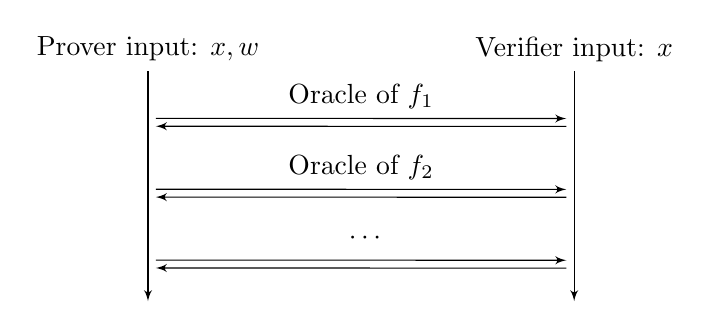
\begin{tikzpicture}[auto, node distance=2.5cm,>=latex']
    \node [rectangle, align=center] (prover) {Prover input: $x, w$};
    \node [rectangle, right=of prover, align=center] (verifier) {Verifier input: $x$};

    \draw[->] (prover) -- +(0, -32mm);
	\draw[->] (verifier) -- +(0, -32mm);

	\draw[->] ([yshift=-6mm, xshift=1mm]prover.south) -- node {Oracle of $f_1$} ([yshift=-6mm, xshift=-1mm]verifier.south);
	\draw[->] ([yshift=-7mm, xshift=-1mm]verifier.south) -- ([yshift=-7mm, xshift=1mm]prover.south);

	\draw[->] ([yshift=-15mm, xshift=1mm]prover.south) -- node {Oracle of $f_2$} ([yshift=-15mm, xshift=-1mm]verifier.south);
	\draw[->] ([yshift=-16mm, xshift=-1mm]verifier.south) -- ([yshift=-16mm, xshift=1mm]prover.south);

	\path (prover) -- (verifier) node[midway, yshift=-26mm] (ellipsis) {$\cdots$};

	\draw[->] ([yshift=-24mm, xshift=1mm]prover.south) --  ([yshift=-24mm, xshift=-1mm]verifier.south);
	\draw[->] ([yshift=-25mm, xshift=-1mm]verifier.south) -- ([yshift=-25mm, xshift=1mm]prover.south);
    \end{tikzpicture}

	\begin{itemize}
		\item Completeness: When $x \in L$, $\Pr[\langle \mathcal{P}(x, w), \mathcal{V}(x) \rangle = 1] = 1$
		\item Soundness: When $x \notin L$, for {\color{red} any} $\mathcal{P}^*$, 
		$\Pr[\langle \mathcal{P}^*(x), \mathcal{V}(x) \rangle = 1] < \epsilon(\kappa)$
	\end{itemize}

\end{frame}

\begin{frame}
    \frametitle{Polynomial Interactive Oracle Proof}
	PIOP: All oracle sent by prover is a polynomial within degree bound.

	\begin{theorem}
	Sound PIOPs are knowledge sound (Lemma 2.3 in HyperPlonk)
	\end{theorem}

	\begin{proof}
	For each oracle of a polynomial with degree $d$, the extractor queries the polynomial at $d+1$ distinct points to extract the polynomial.
	\end{proof}
\end{frame}

\begin{frame}
    \frametitle{IOP of proximity}
	\begin{itemize}
		\item Claim: $x \in \mathcal{L}$
	\end{itemize}

	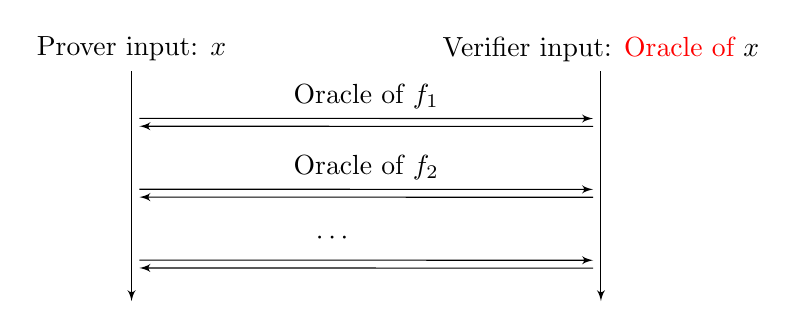
\begin{tikzpicture}[auto, node distance=2.5cm,>=latex']
    \node [rectangle, align=center] (prover) {Prover input: $x$};
    \node [rectangle, right=of prover, align=center] (verifier) {Verifier input: {\color{red} Oracle of} $x$};

    \draw[->] (prover) -- +(0, -32mm);
	\draw[->] (verifier) -- +(0, -32mm);

	\draw[->] ([yshift=-6mm, xshift=1mm]prover.south) -- node {Oracle of $f_1$} ([yshift=-6mm, xshift=-1mm]verifier.south);
	\draw[->] ([yshift=-7mm, xshift=-1mm]verifier.south) -- ([yshift=-7mm, xshift=1mm]prover.south);

	\draw[->] ([yshift=-15mm, xshift=1mm]prover.south) -- node {Oracle of $f_2$} ([yshift=-15mm, xshift=-1mm]verifier.south);
	\draw[->] ([yshift=-16mm, xshift=-1mm]verifier.south) -- ([yshift=-16mm, xshift=1mm]prover.south);

	\path (prover) -- (verifier) node[midway, yshift=-26mm] (ellipsis) {$\cdots$};

	\draw[->] ([yshift=-24mm, xshift=1mm]prover.south) --  ([yshift=-24mm, xshift=-1mm]verifier.south);
	\draw[->] ([yshift=-25mm, xshift=-1mm]verifier.south) -- ([yshift=-25mm, xshift=1mm]prover.south);
    \end{tikzpicture}

	\begin{itemize}
		\item Completeness: When $x \in \mathcal{L}$, $\Pr[\langle \mathcal{P}(x), \mathcal{V}([x]) \rangle = 1] = 1$
		\item Soundness: Let $\delta: [0, 1] \rightarrow [0, 1]$. When $x \notin L$, $\Delta(x, \mathcal{L})$ is relative Hamming distance of $x$ with $\mathcal{L}$. For {\color{red} any} $\mathcal{P}^*$, $\Pr[\langle \mathcal{P}^*(x), \mathcal{V}([x]) \rangle = 1] < \delta(\Delta(x, \mathcal{L}))$
	\end{itemize}
\end{frame}

\end{document}